\chapter{Introduction}
\label{chapter: introduction} 

\looseness -1 \lettrine{I}{n} 2013, U.S data centres consumed 91 billion kilowatt-hour,
which is enough to power every single house in New York City
twice~\citep{Delforge2014DataAssessment, powerforbes}. This is approximately
\SI{5e10}{\kilo\gram} of greenhouse gas emissions, equivalent to the total volume of gas
\emph{emitted by the United Kingdom, the \textrm{5\textsuperscript{$\mathit{th}$}} largest
economy in the world}~\citep{co2emissions}. Due to energy shortages and the difficulty to
produce power at the levels predicted, energy efficiency has, in fact, become a major
issue across the whole computing spectrum, from mobile devices to data centres and
high-performance computing. For this reason, major chip manufacturers and designers, such
as Intel Corp.~\citep{mlawend2} and ARM~\citep{montblanc}, nowadays sacrifice (single
thread) performance for the sake of energy efficiency.  This has been a recent development
(i.e., over the last decade) while scientists have held different opinions throughout the
past four decades regarding performance vs. energy efficiency.  The debate started with
Gordon Moore~\citep{FM1000} advocating for an increase in performance through an increase
in frequency and components complexity (high power), whereas recent reports from Intel
Corp~\citep{mlawend2} suggest many small, simple cores (low power).

% This has been the case over the last decade.  Scientists have held differed opinions
%throughout the past four decades regarding performance vs. energy efficiency, beginning
%with Gordon Moore~\citep{FM1000} advocating for a increase in performance through an
%increase in frequency and components (complexity and high power), whereas recent reports
%from Intel Corp~\citep{mlawend2} suggest many small, simple cores (low power).


%Removed "Search" after Google.

\looseness -1 In addition, large-scale data centres like Facebook~\citep{facebook},
Google~\citep{googlesearch}, Twitter~\citep{twitter}, Amazon~\citep{ec2pricing},
Rackspace~\citep{rack} etc., operate under strict power limitations as energy constitutes
approximately \SI{30}{\percent}~\citep{pdata1,pdata2} of the operating cost of a data
centre. On the one hand, this implies intermittent high loads or software behaviours in
data centres may breach hard power safety
limits~\citep{Bhattacharya:2012:NSS:2410145.2410772}.  On the other hand, despite having
strict power budgets, web-services like Facebook need to deliver services within a certain
time frame otherwise users are likely to leave~\citep{WuDynamo:System}.  Recent study has
shown that marginal delays (of hundreds of milliseconds) in Quality of Service (QoS) can
impact revenue massively~\citep{Eric2009TheSearch}.

To improve energy efficiency (i.e., performance per watt of power consumed) in data
centres, we first need to understand \emph{where?} and \emph{when?} do data centres spend
a lot of time and energy? Several studies concluded that among all the components of a
data centre (servers, cooling, and other infrastructure), the servers consume
approximately \SI{70}{\percent} to \SI{90}{\percent} of the total power consumption
(see~\citep{fblue} and Figure~\ref{fig: breakdown}).  As for the energy consumption within
a server, the CPU~\citep{Lefurgy:2003:EMC:957964.957972} and memory~\citep{6557176,
4658648} are the most dominant consumers~\citep{Barroso2013TheEdition} with each consuming
approximately \SI{30}{\percent}~\citep{5510883}. 

\looseness -1 To improve energy efficiency in data centres, we also need to understand
\emph{how} do data centres spend the power distributed? Several
studies~\citep{Petrucci2015Octopus-Man:Computers, Delimitrou2014Quasar,
Prekas:2015:EPW:2806777.2806848, Barroso2003WebArchitecture} have shown that data centres
like Google and Facebook operate at peak load only for a small fraction of the day
(Figure~\ref{fig: google load1}, $<$ \SI{2}{\hour}), where the power consumption and load
are proportional. However, for the remainder of the day data centres are often
under-utilised (at or below \SI{60}{\percent} mark) while the system power consumption is
greater than \SI{60}{\percent} of the maximum.  My\footnote{In what follows, unless stated
otherwise, I will use the words: I, My, We, Our refer to my exclusive contributions}
thesis focuses on \emph{modelling the performance and power of CPU and memory}
(Part~\rom{2}), the two most power-hungry data centre resources, and proposing
\emph{scheduling strategies to improve energy efficiency} (Part~\rom{3}).

\begin{figure}[t]
    \centering
\begin{tikzpicture}
[
    pie chart,
    slice type={comet}{blu},
    slice type={legno}{rosso},
    slice type={yel}{giallo},
    slice type={sedia}{viola},
    slice type={caffe}{verde},
    pie values/.style={font={\small}},
    scale=2
]

    \pie{Data Centre}{70/comet,30/legno}
    \pie[xshift=3.5cm,values of coltello/.style={pos=1.1}]%
        {Server}{30/caffe,30/yel,40/sedia}

    \legend[shift={(0cm,-1cm)}]{{Server}/comet, {Cooling, etc.,}/legno}
    \legend[shift={(2cm,-1cm)}]{{Disks, Networking, etc.,}/sedia, {Memory}/caffe,
    {CPU}/yel}

\end{tikzpicture}
    \caption[Power consumption breakdown]{Power consumption breakdown in a data centre and server.}
    \label{fig: breakdown}
\end{figure}

\begin{figure}[t] 
    \centering 
    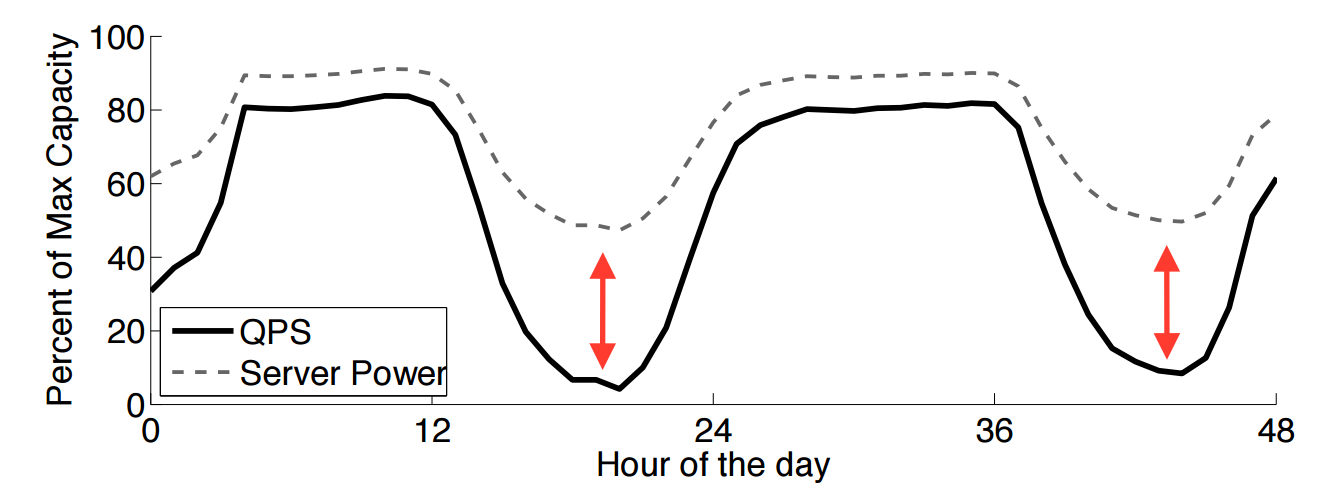
\includegraphics[width=\textwidth]{Chapter0/Figs/octoman.png} 
    \caption[Typical server load and power consumption in Google data centres]{\captitle{Typical 
    server load (in Queries per Second -- QPS) and power consumption in Google data centres.} Workload is given as a percentage 
    of maximum allowed workload.  (Reproduced from~\citep{Meisner2011PowerServices,Bilgir_exploringthe})}
    \label{fig: google load1} 
\end{figure} 


\section{Challenges}% in Modern Data Centres} 

\label{sec: challenges}

We aim to increase data centre energy efficiency by targeting the problem of data centre
particular demands and shared resource contention.  Concretely, we address the following
challenges:


\paragraph{Shared Resource Contention.} Despite significant research
efforts~\citep{Nishtala:2013:ETC:2555754.2555775,Zhuravlev:2013:SES:2498743.2498946,
    Blagodurov:2010:CSM:1880018.1880019, Petrucci:2012:LSE:2387869.2387876,
Petrucci:2015:ETA:2724585.2566618, Zivanovic:2016:LNE:2989081.2989083,
Asifuzzaman:2016:PIS:2989081.2989082}, mitigating shared resource contention on multicore
processors \emph{still} remains a major factor for performance and power loss.  A
multicore server system (schematically shown in Figure~\ref{fig: sharedresource}) has a
set of cores sharing multiple resources like the L2 cache, Last Level Cache (LLC) and DRAM
memory, memory controllers, memory bus, etc.  The latency to fetch data from different
levels of cache hierarchy is known as a miss penalty and is measured in computational
cycles.  The miss penalty is defined as the ratio of the memory access time to the inverse
of core/socket frequency.  Intuitively, one may believe that a higher miss rate would
cause a lower performance (that is, lower instructions per cycle (IPC) or instructions per
second (IPS)).  In addition to shared resource contention, current server systems are also
limited by their memory size~\citep{Zivanovic:2016:LNE:2989081.2989083} and network
saturation~\citep{Guo:2015:PLS:2785956.2787496}. Part~\rom{2} of my thesis focuses on
power and performance prediction in shared resource contention environment.  This is a
challenge for multiple reasons: {\small\circled{1}} It is unclear how to use the hardware
counter information (if any) to understand power and performance trade-offs.
{\small\circled{2}} Some multicore systems in highly complex data
centres~\citep{Mars2013Whare-map} do not necessarily provide all necessary hardware
resource information~\citep{Su:2014:POP:2742155.2742200} to estimate power and performance
accurately. These power and performance estimations are essential to control power
consumption and determine scalability on-the-fly. Part~\rom{3} of my thesis focuses on
scheduling approaches to mitigate shared resource contention to improve energy efficiency.

\paragraph{Data centre particularities.} Regardless of the current computational demand,
server CPUs run at high load ($>$ \SI{60}{\percent}) for short periods, even with
services like Amazon Elastic Compute offered for a small price (under \EUR{5} for 8
virtual CPUs for \SI{1}{\hour}~\citep{ec2pricing}). As shown in Figure~\ref{fig: google
load1}, lower utilisation leads to the disproportionate use of power consumption.  To
improve resource utilisation, intuitively, large-scale data centres like Google and
Twitter wish to collocate batch and interactive workloads on the same
node~\citep{Lo2015Heracles, Dean2013TheScale, Nathuji2010Q-clouds}.  Doing so takes
advantage of the idle periods in interactive applications to amortise idle
power~\citep{Lo2015Heracles}. However, experimental results have shown that collocation of
latency-critical and batch workloads violates Service Level Agreements (SLA) dramatically
due to shared resource contention. For example, Figure~\ref{fig: collocation} shows when a
latency-critical workload is run in isolation and when collocated with a batch workload.
It is clear from the graph that latency-critical workloads are sensitive to shared
resource contention and violate latency even at low loads. For this reason, data centres
tend to run workloads on individual servers instead of collocating.  In Part~\rom{3} of my
thesis, we address the problem of resource utilisation in data centres and show that it is
possible to collocate workloads with intelligent oracles.
        

\begin{figure}[t] 
    \centering
    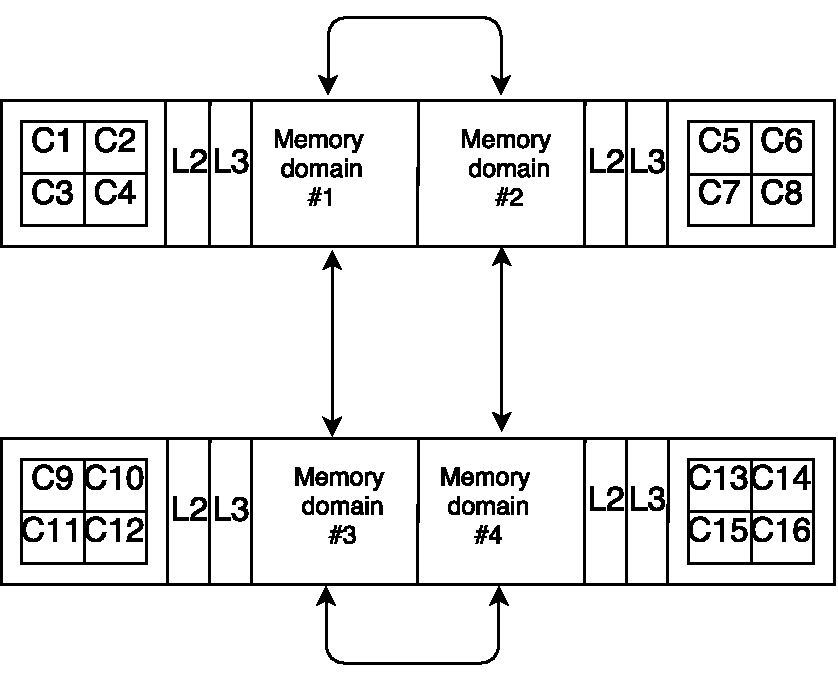
\includegraphics[scale=0.75]{Chapter0/Figs/Sharedresource.pdf} 
    %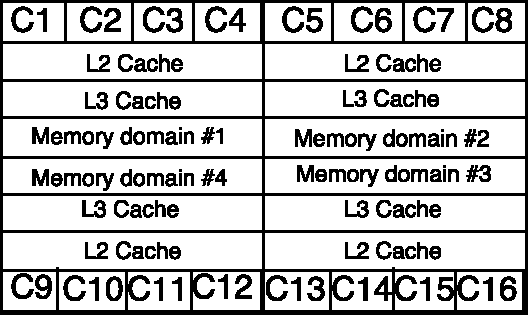
\includegraphics[scale=0.75]{Chapter0/Figs/SHARED_RESOURCE.pdf} 
    \caption[High level view of multicore server system]{\captitle{High level view of multicore server system.} Each domain contains 4 cores with a shared L2 and LLC per domain.} 
    \label{fig: sharedresource} 
\end{figure}

\begin{figure}[htb] 
    \centering
    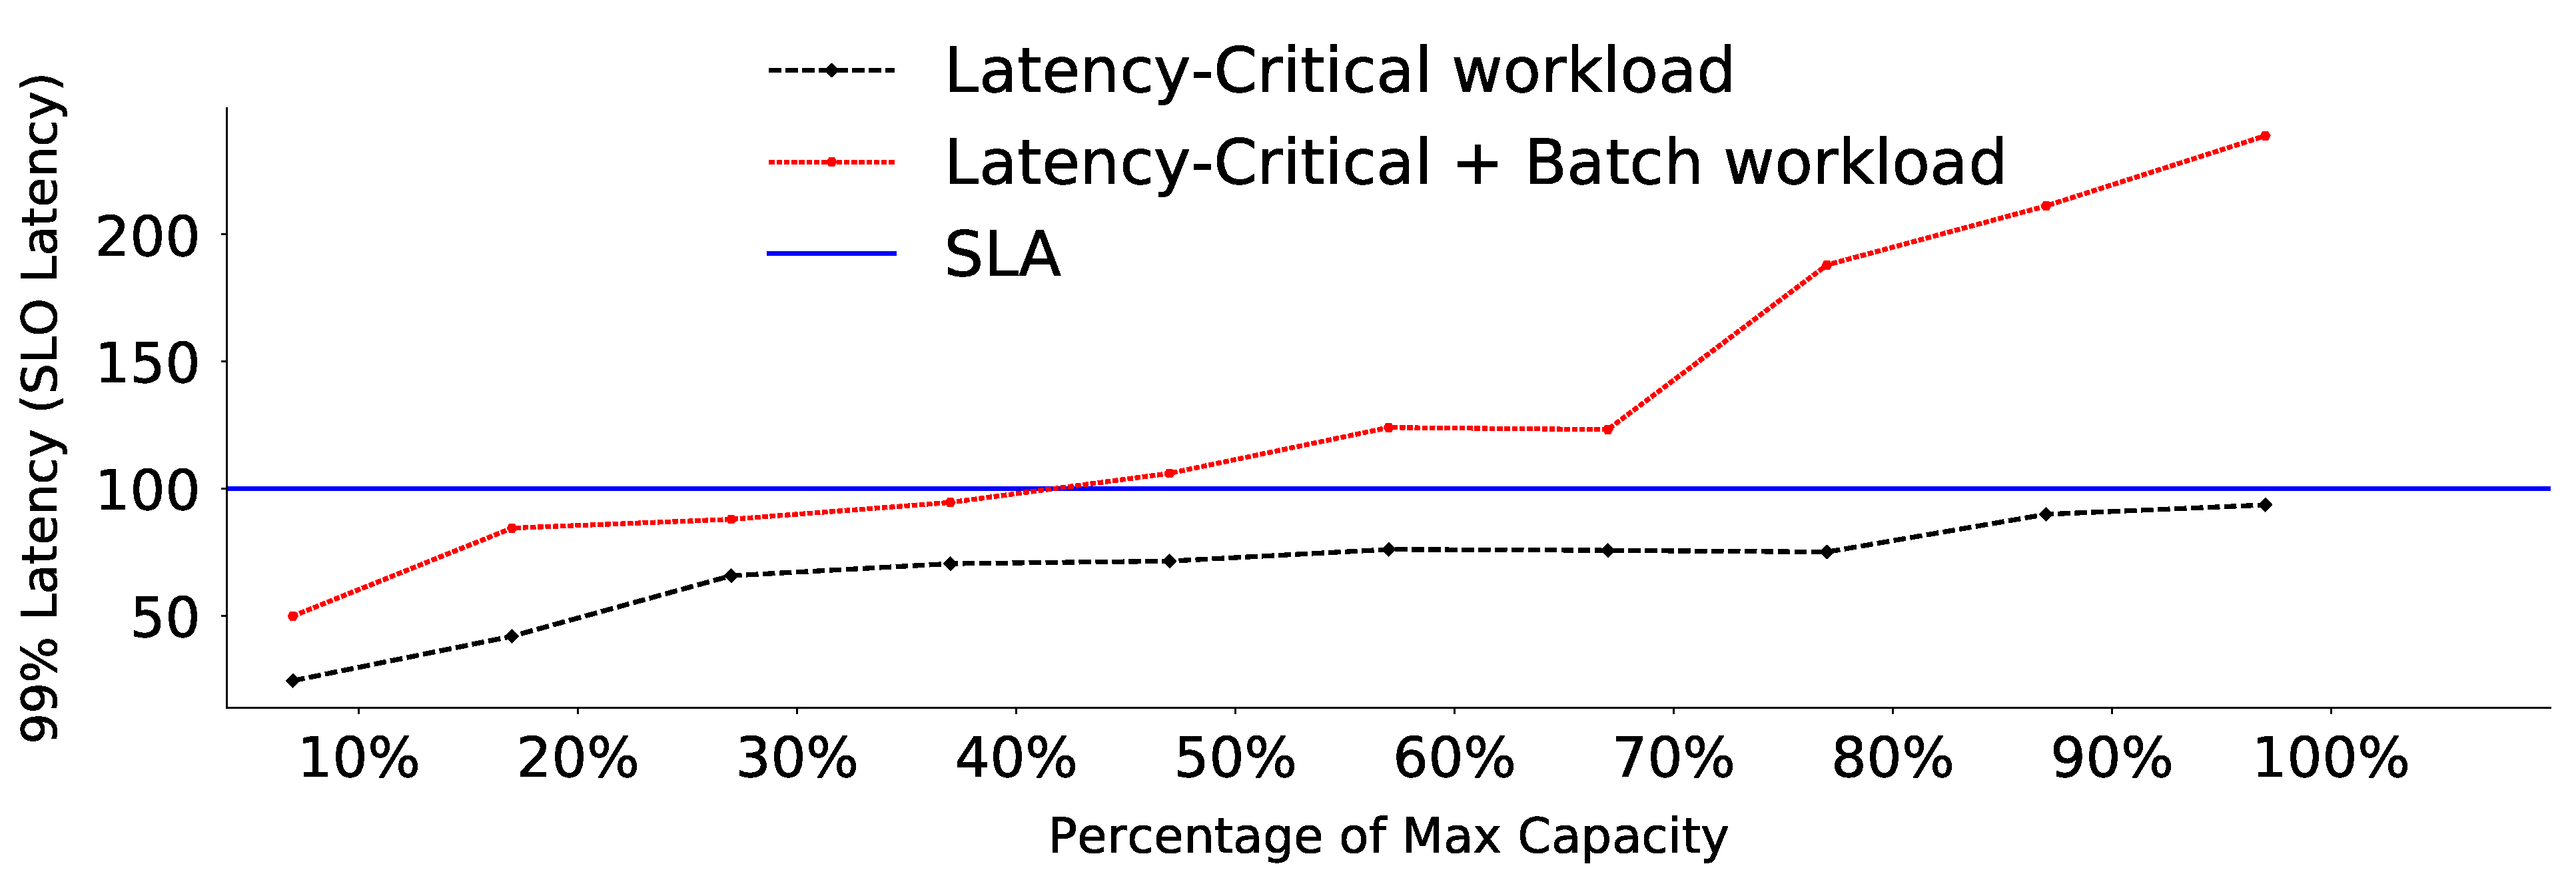
\includegraphics[width=\textwidth]{Chapter0/Figs/colloc.eps}
    \caption[Colloation of latency-critical and batch workload]{\captitle{Collocation of latency-critical and batch workload.} Percentage SLO for latency-critical workload (Web-Search) when run in isolation and when collocated with a batch workload.}
    \label{fig: collocation}
\end{figure}

\looseness -1 \paragraph{Transition to Heterogeneous processors.} Despite power being a
rarely found additional resource in today's data centres, it is often an under-optimised
resource.  Even with advanced hardware power techniques, commercially available processors
cannot reduce the power consumption below the minimum operating power
consumption~\citep{Halpern2016MobileSatisfaction, Wong2012KnightShift:Heterogeneity}.
This has been the case for a very long time, and, as a result, the computing spectrum is
moving towards \emph{\het \muc processors}~\citep{JanapaReddi2010WebCores,
Chitlur2012QuickIA:Prototypes, Guevara2013NavigatingMechanisms, 7855903}.  Heterogeneous \muc
processors are a combination of high-performance and high power consumption processors,
and low performance and low power processors with a single instruction set architecture
(ISA). 


On the one hand, the in-order processor (low performance) is interesting as it compromises
performance to reduce the minimum operating power consumption during periods of low
activity and improves power proportionality~\citep{JanapaReddi:2010:WSU:1816038.1816002}
and therefore, we deploy a heterogeneous platform in the scheduling solution presented in
Part~\rom{3}.  For this reason, these processors are gaining immense
popularity~\citep{montblanc, montblanc2, montblancproto, Rajovic:2013:SCC:2503210.2503281,
armmuscle} in both supercomputers and data centre community. On the other hand, to build a
prediction model to estimate performance and power (Part~\rom{2}) on a heterogeneous
platform is a challenge for multiple reasons: {\small \circled{a}} It is unclear if there
exist (same) hardware counters on both out-of-order~\citep{Cristal:2004:OCP:1072448.1072456} and
in-order~\citep{JanapaReddi:2010:WSU:1816038.1816002} processors to estimate performance
and power.  {\small \circled{b}} It is unclear how the performance and power varies across
processor types and different hardware control settings.

\nomenclature[z-ISA]{ISA}{Instruction Set Architecture}

\looseness -1 \paragraph{Scheduling workloads.} Recent
work~\citep{Zhuravlev:2013:SES:2498743.2498946, Zhuravlev:2012:SST:2379776.2379780,
Mars:2011:BIU:2155620.2155650, Mars:2011:DCC:1944862.1944887, Yang2013Bubble-flux} have
shown that traditional power management practices and CPU utilisation measures are
unsuitable to drive task management for modern data centre workloads. This is because the
nature of workloads run on data centres is transitioning from batch workloads to
latency-critical.  Prior schemes, like OS-level dynamic voltage and frequency scaling
(DVFS), work well to deliver long-term performance for batch workloads, but they can
severely hurt the QoS of interactive data centre workloads.  Part~\rom{3} of my thesis
addresses the problem of meeting SLA requirements of latency-critical workloads while
improving energy efficiency.

\section{Outline of thesis} 

\label{section: outline-of-thesis}

\looseness -1 The two most significant contributions of my research are as follows.
{\small\circled{1}} An architecture and application agnostic power and performance
estimation model to control \emph{on-the-fly} server power consumption and performance
delivered.  {\small\circled{2}} A hybrid scheduling approach to manage resource allocation
on \het server processors to improve resource utilisation while meeting performance
guarantees.  Below are details of the research questions and contributions.

\paragraph{Estimate and control performance and power.} Large scale complex and
heterogeneous data centres are often constrained to external power budget and strict
performance SLA.\footnote{In this context, heterogeneous indicates different homogeneous
processors~\citep{Mars2013Whare-map} on a single server system.} On the one hand,
maintaining SLA is important as it drives the capital investment. On the other hand, not
maintaining external power budgets penalises the budget. This performance and power
trade-off in data centres raises the need to estimate performance and power at different
hardware settings to ensure power budgets and SLA agreements are met.  Prior
state-of-the-art solutions addressed the need for a model on a single architecture while
considering the contention for cache, memory, and numerous processors components.  All
these factors are essential in building a model, and prior solutions address some parts of
the problem.  However, we were interested in answering the question \emph{``How do we
build power and performance models that can be scalable and can integrate seamlessly in a
dynamic data centre?''}

In Chapter~\ref{chap: REPP}, we introduce a systematic methodology to build models to
predict power and performance at DVFS and idle-states at runtime for a \textit{single
core}  and \textit{\muc} processors (REPP: Runtime Estimation of Performance and Power).
We suggest after extensive experimentation that accurate power and performance models can
be built for modern architectures using basic hardware performance monitoring
counters (PMCs)~\citep{6651797}. The PMCs chosen to build the models are available on all major
architectures.  Extensive real-machine experimentation results of batch workloads on
multiple architectures results has shown that the models predict power and performance
with at least \SI{93}{\percent} accuracy. 


\looseness -1 Taking into account strict power restrictions data centres need to sustain,
utilising all cores in idle periods is not beneficial. Therefore, data centres are
shifting the trend towards consolidation workloads and shutting down cores to improve
energy efficiency.  Chapter~\ref{chap: REPP} does not address the power consumption or
performance characterisation of workloads with certain servers shutdown. Precisely,
Chapter~\ref{section: REPP-C} extends REPP to introduce a mechanism to estimate
performance and power with core consolidation, DVFS, and idle-states (Runtime Estimation
of Performance and Power with Core Consolidation -- REPP-C) in multicore architectures. At
it's core REPP-C solves a multi-objective problem by first scheduling workloads from
consolidated cores to maximise energy efficiency. Next, it models the impact of
performance and power due to core shutdown. 

\paragraph{Addressing resource utilisation.} With the nature of applications running on
data centres changing, collocating workloads that contend for shared resources is
difficult (see Figure~\ref{fig: collocation}).  This, in large-scale, translates to
selecting either performance or power objective which are tightly coupled. Enabling higher
power savings may imply performance SLA is violated, whereas lower utilisation implies bad
power usage. 


\looseness -1 Prior approaches were based on a static oracle (based on offline profiling)
for a given architecture to migrate across different configurations (a configuration may
be defined as an iso-latency~\citep{Lo2015Heracles} policy to control the DVFS
state~\citep{Kasture2015Rubik} or cores
allocated~\citep{Petrucci2015Octopus-Man:Computers} and DVFS state, network bandwidth
allocation~\citep{NCAP:HPCA}, etc.) to satisfy performance guarantees of interactive
workloads.  This is a problem for two reasons.  {\small\circled{1}} Applications have
different resource requirements to satisfy SLA at a given load.  This, in part, is due to
workloads having different characteristics.  {\small\circled{2}} With an erratic
application behaviour or a sudden spike in external load, the reaction time is
proportional to the number of configurations available, thereby they have a much higher
potential to have a significant performance loss. These schedulers are necessary and
essential to address some parts of the problem for a given application on an architecture.
However, we were interested in answering the question \emph{``How do we detect on-the-fly
the best configurations for a latency-critical job on any architecture?''} In
Chapter~\ref{chapter: hipster},  we introduce a novel method based on an oracle and
reinforcement learning to manage interactive and batch workloads.  Our approach provides
the interactive application with ``just enough'' resources to meet the real-time
performance constraint, while the remaining resources are given to batch workloads to
maximise throughput. After extensive experimentation, we argue that using only an single
oracle is inefficient in today's data centres and demonstrate that our results outperform
state-of-the-art schedulers. 


\looseness -1 The rest of the thesis is structured as follows: Chapter~\ref{chap:
infrastructure} provides a background on the performance and power monitoring tools, the
different architectures used, their hardware capabilities and power efficiency details.
Chapters~\ref{chap: REPP} and~\ref{section: REPP-C} describe the performance and power
modelling methodology and control technique for multicore architectures.
Chapter~\ref{chapter: hipster} introduces a scheduling technique to improve resource
efficiency in data centres while meeting the performance guarantees of interactive
workloads.  Chapter~\ref{chap: relatedwork} discusses the related work, chapter~\ref{chap:
finalconc} concludes the thesis, and chapter~\ref{chap: futurework} describes the future
work.

